%% Appendix (included by paper.tex in the arXiv and submission-appendix builds).
%% Keep the \apprefFallback table in paper.tex in step with the labels below.

\setcounter{figure}{0}
\renewcommand{\thefigure}{A\arabic{figure}}
\setcounter{table}{0}
\renewcommand{\thetable}{A\arabic{table}}
% Distinct link targets, so that Table A5 does not link to Table 5 in the arXiv version.
\renewcommand{\theHfigure}{A\arabic{figure}}
\renewcommand{\theHtable}{A\arabic{table}}

\begin{figure*}[t]
\centering
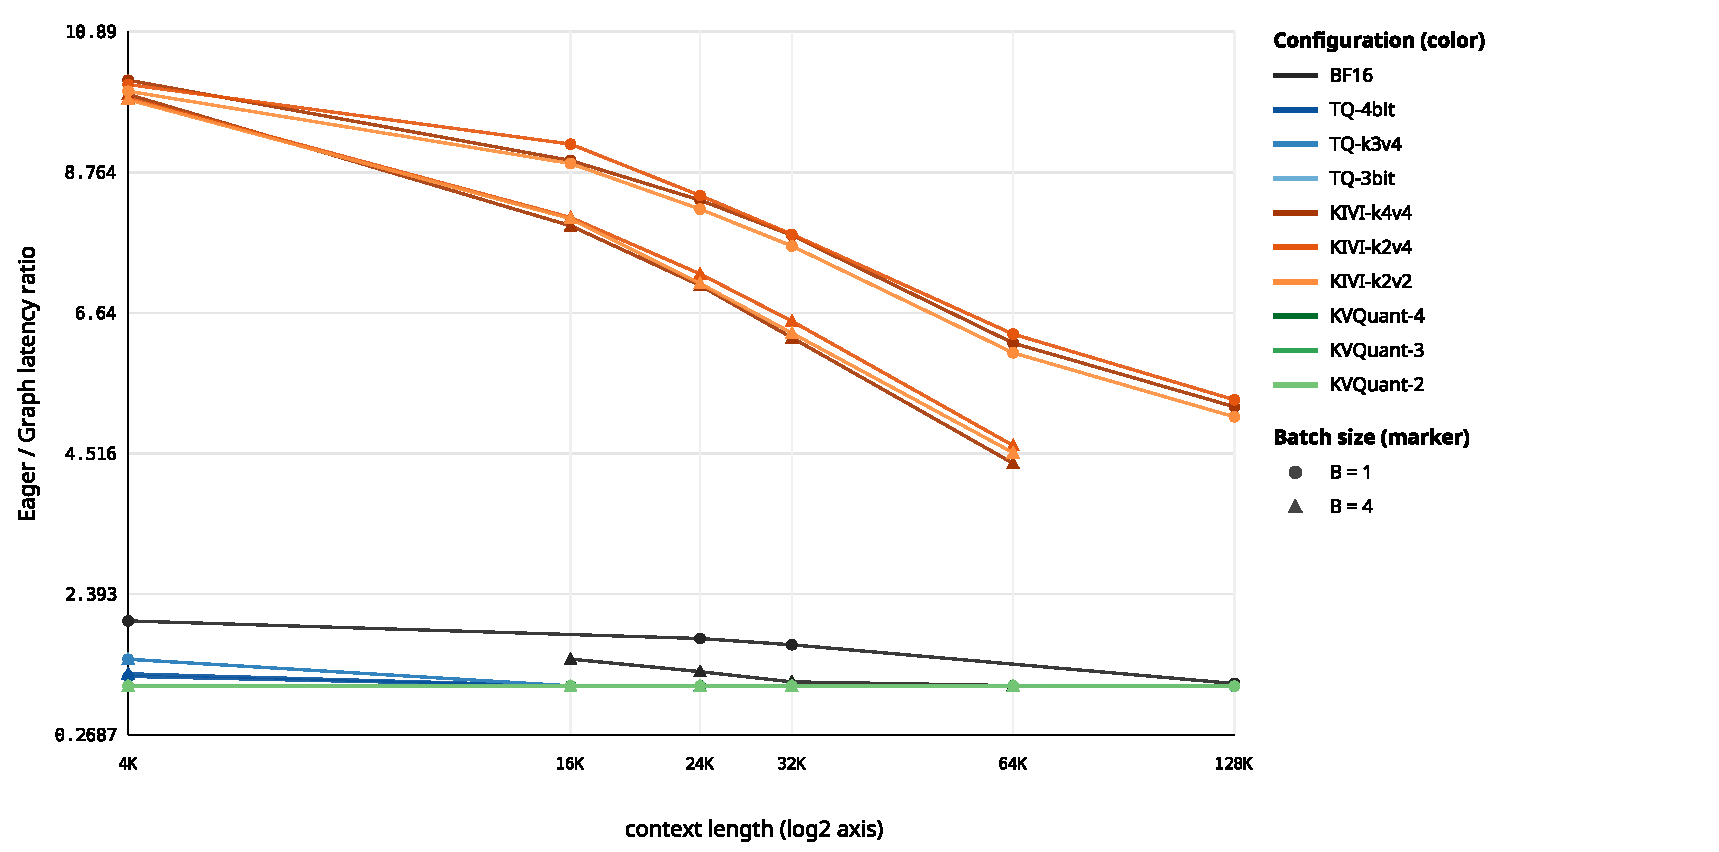
\includegraphics[width=\textwidth]{figures/fig2_graph_ab_ratio.pdf}
\caption{Eager-to-Graph latency ratio versus context for each configuration at $B = 1$ and $B = 4$ (within-configuration mechanism experiment).
KIVI's ratio starts near 10 and declines with context.
BF16 starts near 2.
TurboQuant\ported{} and KVQuant stay close to 1.}
\label{fig:graph}
\end{figure*}

\section{Reproducibility}
\label{app:repro}

As in the main paper, TurboQuant\ported{} denotes TurboQuant as ported, with split-KV count 4 (Section~\mainref{sec:impl}).
The results were produced at repository commit \anon{0641de4b}.
The study used model \hash{meta-llama/Llama-3.1-8B-Instruct} at revision \hash{0e9e39f249a16976918f6564b8830bc894c89659}.
Performance runs used measurement container \anon{\hash{sha256:059bc9be89387369d7de9e3e9b26d85b6e9902c41e7dbf002ebc45edd188fb7e}}, and quality runs used its derivative \anon{\hash{sha256:1d8056643bf001fb83ee19e6bb19ec93379c296f2be6ba02e907d0b2f4ecca32}}.
Performance data are identified by the tag \anon{\hash{perf-freeze-20260917-83536c37-r1}}.
The hardware manifest, per-run configuration, raw samples, and five independent process measurements per point are retained under content-addressed roots with indefinite retention: full-scan wall-clock root \anon{\texttt{5605558b\ldots}}, profiler root \anon{\texttt{641fc02d\ldots}}, modeling root \anon{\texttt{05d5c4e8\ldots}}, and joint-results root \anon{\texttt{2d609efb\ldots}}.
The KIVI and KVQuant source patches are stored in the repository with their manifests.
Two CPU-only packages run without a GPU or network access: the modeling package (Python standard library only) regenerates the modeling audit, figures, and predictor examples, and the joint-results package (Python with pyarrow) regenerates the per-stage outcome table, the joined quality--performance table, and the empty table of qualified configurations byte-for-byte.
The joint-results package also carries the frozen inputs of Tables~\mainref{tab:alloc}--\mainref{tab:latency} and Figure~\mainref{fig:samework}a; the frozen columns of Table~\mainref{tab:traffic} computed from it match the table digit for digit.
The v1.0 release notes and manuscript use the numbering of an earlier version of this paper; Table~\ref{tab:numbering} maps it to this version.

Post-hoc analyses.
The analyses of Appendices~\ref{app:ceilings}, \ref{app:diagnostics}, and~\ref{app:kvquant} were defined after the results were known and read only the frozen roots above; none reruns a timing scan or a quality run.
Their code and outputs are sealed under the same retention scheme: traffic model, ceilings, bandwidth, elasticity, capacity, and decomposition \anon{\texttt{3dc84c64\ldots}}; kernel breakdowns from the existing traces \anon{\texttt{c347e20a\ldots}}; the Nsight diagnostics of Appendix~\ref{app:diagnostics}, raw \anon{\texttt{4cdbb3ae\ldots}} and analysis \anon{\texttt{39efeb1c\ldots}}; the KVQuant quality exclusion record \anon{\texttt{47296f7c\ldots}}; the final-revision analyses (cache-only ceiling, KIVI kernel breakdown) \anon{\texttt{b0969338\ldots}}; and KIVI's adjusted ratio $S_{\mathrm{adj}}$ \anon{\texttt{1998be3e\ldots}}.
The post-hoc code is on the repository's main branch, not in the v1.0 release; rerunning its CPU analyses on the retained roots reproduces their sealed tables and figures unchanged.
Every number that the v1.0 packages do not contain, including the post-hoc columns of Table~\mainref{tab:traffic} and panel b of Figure~\mainref{fig:samework}, comes from these artifacts.

\begin{table}[t]
\caption{Table, figure, and section numbers in the v1.0 release (manuscript and release notes) and in this version.}
\label{tab:numbering}
\vskip 0.1in
\centering
\footnotesize
\setlength{\tabcolsep}{3pt}
\begin{tabular}{@{}L{3.7cm}L{4.0cm}@{}}
\toprule
v1.0 & This version \\
\midrule
Table 5 (candidate scores) & Table~\ref{tab:candidates} \\
Table 6 (model D errors) & Table~\ref{tab:modelD} \\
Table 7 (perplexity) & Table~\mainref{tab:ppl}; KVQuant rows in Table~\ref{tab:kvq-ppl} \\
Table 8 (LongBench v2) & Table~\mainref{tab:lbv2} \\
Table 9 (joint outcome) & Table~\mainref{tab:joint} \\
Figure 2 (eager/Graph ratio) & Figure~\ref{fig:graph} \\
Figure 3 (held-out predictions) & Figure~\ref{fig:heldout} \\
Sections 4.1--4.3 (modeling) & Section~\mainref{sec:model} and Appendix~\ref{app:modeling} \\
Section 6.2 (reproducibility) & Appendix~\ref{app:repro} \\
Section 6.3 (conclusions) & Section~\mainref{sec:conclusions} \\
Tables 1--4, Figure 1, Sections 1--3 and 5 & unchanged; Figure~\mainref{fig:samework} adds the post-hoc panel b \\
\bottomrule
\end{tabular}
\end{table}

Modeling.
Beyond the limits in Appendix~\ref{app:modeling}, fold-level coefficient vectors were not saved, so held-out predictions are tied to the stored out-of-fold table and the fitting code.

Run accounting.
The full scan comprises 2,670 planned runs (534 points $\times$ 5 processes): 2,205 completed runs and 465 predicted capacity-infeasible.
Thirty-eight runs were replaced after infrastructure failures, each linked to the run it replaces, and no valid, slow, or unstable observation was rerun; output checksums, kernel paths, and allocations agree across processes.
In the eager-versus-Graph experiment, 10 of 120 conditions were predicted infeasible and 105 were stable; five eager conditions (three BF16, two TQ-3bit) exceeded the 3\% CV threshold and were kept as unstable, excluded from fitted comparisons, and not rerun.
The quality--performance join matches runs by exact configuration identity and retains all 2,670 planned runs, with no unmatched or duplicated identities.

Artifact availability.
The code, configurations, and method patches are released at \anonurl{\RepoURL} as release tag v1.0 (default branch) under the Apache-2.0 license; vendored and patched third-party code keeps its upstream terms, listed in the repository's NOTICE file.
The protocol, decision records, and full research history are on the main branch at commit \anon{0641de4b}.
The two CPU reproduction packages are released as GitHub Release assets.
The raw measurements are available from the authors on request.
Model weights are gated under the Llama 3.1 Community License and are not redistributed.

Modeling package (Python standard library only), run from the package root:

{\scriptsize
\begin{verbatim}
python3 reproduce.py reproduce --package . \
    --output <output_dir>
\end{verbatim}
}

Joint quality--performance package (Python with pyarrow), run from the package root:

{\scriptsize
\begin{verbatim}
python3 reproduce.py --reproduce . \
    --output <output_dir>
\end{verbatim}
}

In both cases \texttt{<output\_dir>} must not exist yet.
\section{Protocol timeline}
\label{app:timeline}

\begin{center}
\footnotesize
\begin{tabular}{@{}L{1.75cm}L{5.85cm}@{}}
\toprule
Date (2026) & Event \\
\midrule
Jul 22 & Scope, model, and performance measurement protocol fixed; post-performance quality protocol (stages, gates, margins) preregistered \\
Jul 25--31 & Measurement container fixed; per-method and unified validation gates passed \\
Aug 22--26 & Pilot scan; knee-densification design (84 adaptive contexts) frozen and executed; an earlier blocked pilot attempt contributed no timing \\
Aug 26--30 & Eager/Graph mechanism experiment; profiler subset \\
Aug 31--Sep 16 & Full scan executed; wall-clock primary analysis completed; an earlier stopped scan attempt contributed no timing \\
Sep 16--17 & Modeling and CPU reproduction package \\
Sep 17--18 & Performance data frozen; exact quality inputs and mechanical choices fixed \\
Sep 19 & Correctness stage: all ten configurations fail cross-batch invariance; BF16 diagnosis \\
Sep 19 & Physical-$B = 1$ amendment approved, before any perplexity score \\
Sep 19--21 & Fast perplexity \\
Sep 21--27 & Full perplexity (KIVI-k4v4) \\
Sep 27--Oct 2 & LongBench-E (KIVI-k4v4) \\
Oct 2--4 & LongBench v2 no-CoT (KIVI-k4v4) \\
Oct 4 & Joint validation and scoped quality--performance join \\
Oct 4--5 & Post-hoc review analyses on the frozen data and Nsight diagnostics (Appendices~\ref{app:ceilings}, \ref{app:diagnostics}, and~\ref{app:kvquant}); no timing scan or quality run \\
\bottomrule
\end{tabular}
\end{center}

The first full-scan summary computed ratios from CUDA-event medians.
A later append-only analysis re-derived the preregistered wall-clock statistics from the same raw files without rerunning any timing, and all timing numbers in this paper use wall-clock time.

\section{Traffic model, ceilings, and effective bandwidth (post hoc)}
\label{app:ceilings}

Everything in this appendix was defined after the results were known.
It uses the frozen wall-clock process medians, the byte accounting of Section~\mainref{sec:ratios}, and the Nsight Compute profiles, which flush caches before every kernel replay and lock base clocks, so their DRAM bytes are cold-cache counts.

\textit{Traffic model.}
For configuration $m$ at $(B, L)$ we model the DRAM traffic of one decode step as $D_m(B, L) = N_f(B, L) + \alpha_m C_m(B, L)$, where $C_m$ is the allocated cache and $\alpha_m$ is the cache-path DRAM per allocated byte at the profiled point ($B = 1$, 128K): 1.01 for BF16, 0.77--0.81 for TurboQuant, 1.13--1.21 for KIVI, and 1.48--1.81 for KVQuant, whose key-path kernels the model counts as cache traffic (below).
The non-cache term $N_f = n_0 + n_1 B (L + 1)$ is fit per family to every $B = 1$ profile of the family: $n_0 = 15.1$ GB and $n_1 \approx 0$ for BF16 and TurboQuant, and $n_0 = 15.3$ GB with $n_1 = 12.6$ and 12.1 KB per sequence token for KIVI and KVQuant, whose kernels write logits-sized intermediates; extending $n_1$ to $B > 1$ assumes this work is per sequence.
At the twelve profiled points other than 128K, the cache term, which is out of sample there, is within 2.8\% of the measurement and the total within 0.5\%.
Post-hoc Nsight Compute profiles of BF16, TQ-4bit, and KIVI-k4v4 at $B = 8$, 32K and $B = 16$, 16K test the extension to larger batches: the modeled total is within 3.1\% of the measurement and the non-cache term within 2.6\%; the cache term is within 1.2\% for BF16 and TQ-4bit, and the model underestimates KIVI's cache-path traffic by 4.1--4.6\%.

\textit{KVQuant classification.}
The frozen classification assigns kernel names containing ``rope'' to other model work, which put KVQuant's key-score kernels (\hash{VecQuant[2-4]MatMulKernelNUQPerChannelTransposedRopeMHABatchedFusedOpt}, which read the packed key cache) and its sparse-key kernel (\hash{SPMV\_ATOMIC\_ROPE\_BALANCED}) outside the cache path.
Moving them in adds 3.53, 3.00, and 2.46 GB at 128K for KVQuant-4, -3, and -2 (Table~\ref{tab:kvq-traffic}) and makes the family's non-cache fit consistent across bit widths (largest residual 0.8\% of total traffic, against 3.0\% before).
No other family changes.
Table~\mainref{tab:traffic} keeps the frozen values; the traffic model, the ceilings, the elasticities, and the decomposition use the reclassified KVQuant traffic.

\begin{table}[t]
\caption{KVQuant at $B = 1$, 128K: frozen classification (Table~\mainref{tab:traffic}) $\to$ key-score and sparse-key kernels counted in the cache path (post hoc).
Bandwidth as in Table~\mainref{tab:traffic}, as a share of peak.}
\label{tab:kvq-traffic}
\vskip 0.1in
\centering
\footnotesize
\setlength{\tabcolsep}{3pt}
\begin{tabular}{@{}l>{\raggedleft\arraybackslash}p{1.55cm}>{\raggedleft\arraybackslash}p{1.45cm}>{\raggedleft\arraybackslash}p{1.45cm}>{\raggedleft\arraybackslash}p{1.45cm}@{}}
\toprule
 & Cache-path DRAM (GB) & $r_{\mathrm{DRAM}}$ & $A$ & Cache-path BW (\%) \\
\midrule
KVQuant-4 & 4.54 $\to$ 8.08 & 3.82 $\to$ 2.15 & 0.82 $\to$ 1.46 & 2.0 $\to$ 3.6 \\
KVQuant-3 & 3.78 $\to$ 6.78 & 4.60 $\to$ 2.56 & 0.88 $\to$ 1.58 & 1.7 $\to$ 3.0 \\
KVQuant-2 & 3.16 $\to$ 5.62 & 5.50 $\to$ 3.09 & 1.01 $\to$ 1.79 & 1.4 $\to$ 2.4 \\
\bottomrule
\end{tabular}
\end{table}

\textit{Ceilings.}
$S_{\mathrm{eq}} = D_{\mathrm{BF16}} / D_m$ uses the as-ported traffic.
The ideal cache traffic $D_{\mathrm{ideal,cache},m} = \alpha_{\mathrm{BF16}} C_m$ assumes the method reads its allocation as efficiently as BF16 reads its own ($A = 1$).
$S_{\mathrm{cache}}$ (Section~\mainref{sec:traffic}) keeps BF16's measured non-cache time, $T_{\mathrm{BF16}} - D_{\mathrm{cache,BF16}} / BW_{\mathrm{eff,BF16}}$ with $BW_{\mathrm{eff,BF16}}$ at the same batch size from Table~\ref{tab:bweff} (at least 11.3 ms at every point), and moves $D_{\mathrm{ideal,cache},m}$ at $BW_{\mathrm{peak}} = 1{,}792$ GB/s, NVIDIA's published figure, which the Nsight Compute device attributes reproduce (14.001 GHz memory clock $\times$ 2 $\times$ 512-bit bus).
Excluding decode workspace and padding from $C_m$ raises TurboQuant's $S_{\mathrm{cache}}$ from 1.02--1.70 to 1.02--1.88 and changes the others by at most 0.01.
For comparison, the roofline ceiling $S_{\mathrm{roof}} = T_{\mathrm{BF16}} \cdot BW_{\mathrm{peak}} / (N_{\mathrm{BF16}} + D_{\mathrm{ideal,cache},m})$, 1.37--2.78 at the same-work points, also lets the non-cache work, mostly the 15.1 GB of weights, run at peak bandwidth, so it includes speedups unrelated to the cache: at $B = 1$, 4K it is 1.37--1.39, although the cache path is only 2.9\% of BF16's step time and $S_{\mathrm{cache}}$ is 1.02.
BF16 itself moves its modeled traffic at 72--85\% of peak at the same-work points.

\textit{Effective bandwidth.}
Total: total decode DRAM at 128K over the 128K step time.
Cache path: $(D_{\mathrm{cache}}(128\mathrm{K}) - D_{\mathrm{cache}}(4\mathrm{K})) / (T(128\mathrm{K}) - T(4\mathrm{K}))$ at $B = 1$, with $D_{\mathrm{cache}}(4\mathrm{K})$ measured for BF16, TQ-4bit, and KIVI-k4v4 and modeled otherwise.
Using $D_{\mathrm{cache}}(128\mathrm{K})$ alone in the numerator gives 92.2\% for BF16 and 8.0--12.9\% for KIVI.

\textit{Elasticity.}
At each $(B, L)$ where all three configurations of a family were measured, we regress $\log T$ (point medians) on $\log C_{\mathrm{alloc}}$ across the bit widths, and the same regression of the logarithm of modeled traffic gives the slope expected if latency were proportional to traffic.
A threshold fixed before any slope was computed keeps the 40 points where modeled cache traffic is at least 25\% of the total (92 fall below it; 30 lack a configuration).
Pooled within-point slopes are 0.142 [0.140, 0.148] for KIVI (expected 0.304), $-0.057$ [$-0.057$, $-0.055$] for KVQuant (0.242), and 1.243 [1.228, 1.264] for TurboQuant\ported{} (0.553); the intervals come from 2,000 bootstrap draws over the five process sessions and reflect timing noise only.
TurboQuant's bit widths also select different kernel specializations, so its slope mixes byte and kernel effects.

\textit{Steady-state capacity.}
Steady-state memory is the weights, the allocated cache including its persistent workspace, the endpoint workspace, and the CUDA Graph pool, all from the preregistered feasibility formula; the transient is the prefix-construction peak (MLP intermediates of the unchunked prefill), the prefix control tensors, and KVQuant's prefix-packing scratch.
All values are predictions.
Steady state admits 505 of the 534 grid points (end to end: 441), and no end-to-end-feasible point is infeasible in steady state.

\begin{table}[t]
\caption{Effective cache-path bandwidth $BW_{\mathrm{eff}}$ (GB/s) from the decomposition $T = c_0 + D_{\mathrm{cache}} / BW_{\mathrm{eff}}$ fitted across contexts at each batch size (Section~\mainref{sec:model}; post hoc).}
\label{tab:bweff}
\vskip 0.1in
\centering
\footnotesize
\setlength{\tabcolsep}{4pt}
\begin{tabular}{@{}lrrrrr@{}}
\toprule
Configuration & $B=1$ & $B=2$ & $B=4$ & $B=8$ & $B=16$ \\
\midrule
BF16 & 1602 & 1639 & 1649 & 1653 & 1665 \\
TQ-4bit\ported{} & 14 & 28 & 58 & 113 & 208 \\
TQ-k3v4\ported{} & 19 & 39 & 78 & 146 & 212 \\
TQ-3bit\ported{} & 14 & 29 & 60 & 114 & 177 \\
KIVI-k4v4 & 229 & 342 & 455 & 478 & 477 \\
KIVI-k2v4 & 199 & 305 & 419 & 443 & 443 \\
KIVI-k2v2 & 142 & 229 & 321 & 379 & 379 \\
KVQuant-4 & 70 & 66 & 78 & 103 & 60 \\
KVQuant-3 & 57 & 54 & 64 & 91 & 50 \\
KVQuant-2 & 47 & 44 & 52 & 53 & 35 \\
\bottomrule
\end{tabular}
\end{table}

\section{Profiler diagnostics (post hoc)}
\label{app:diagnostics}

\textit{TurboQuant geometry and upstream parity.}
Nsight Systems traces (Graph mode, eight replays) and Nsight Compute reports show the stage-1 grid $(B, 32, 4)$ with 32 threads per CTA for all three configurations.
At $B = 1$ its share of traced GPU kernel time is 55.7\% at 4K, 90.6\% at 32K, and 97.2\% at 128K (TQ-4bit, as ported).
Our kernel source matches vLLM v0.25.1 except for imports, and the adapter launches it with the upstream parameters (stage 1: four tokens per tile, one warp, one stage; stage 2: four warps, two stages) except the split count: vLLM's \texttt{tq\_max\_kv\_splits\_for\_cuda\_graph} defaults to 32, while our port, and the G1 reference fixtures, use 4.

\textit{Split-count diagnostic.}
In the measurement container, with the Full Scan execution repository and the same session construction (BF16 restores its prefix snapshot; compressed configurations rebuild the cache from the logical prefix), we traced eight Graph replays per point with the split count at 4 (as ported) and at 32 (Table~\ref{tab:split}).
The 32-split runs swap the split constant and a caller-owned scratch only inside each decode call; in all 33 traced runs, the 12 with 32 splits included, the historical cache and its pointers were unchanged, the adapter fingerprint validated, and outputs were finite (worker checks sealed with the analysis, root \anon{\texttt{39efeb1c\ldots}}).
These checks cover finiteness and cache integrity only; we did not verify that 32-split outputs agree numerically with the 4-split path.
$B = 8$ at 128K is infeasible, so $B = 8$, 48K replaces it.
As-ported traced kernel time per step agrees with the frozen wall-clock medians to within 2.5\%.

\begin{table}[t]
\caption{TurboQuant split-count diagnostic (Nsight Systems, median of eight replays): stage-1 and whole-step GPU kernel time per decode step (ms) with 4 (as ported) and 32 splits, and the 32-split step time over BF16's at the same point.
Profiler observations of GPU kernel time, not wall-clock benchmark timing.}
\label{tab:split}
\vskip 0.1in
\centering
\footnotesize
\setlength{\tabcolsep}{3pt}
\begin{tabular}{@{}lrlrrrrr@{}}
\toprule
 & & & \multicolumn{2}{c}{Stage 1} & \multicolumn{2}{c}{Step} & \\
Config & $B$ & $L$ & 4 & 32 & 4 & 32 & 32/BF16 \\
\midrule
TQ-4bit & 1 & 32K & 113.4 & 14.4 & 124.4 & 26.4 & 1.89 \\
TQ-4bit & 1 & 128K & 448.1 & 56.4 & 459.4 & 70.0 & 3.16 \\
TQ-4bit & 8 & 32K & 108.9 & 39.7 & 122.3 & 54.5 & 1.68 \\
TQ-4bit & 8 & 48K & 163.1 & 61.4 & 177.2 & 77.9 & --- \\
TQ-k3v4 & 1 & 32K & 76.6 & 10.4 & 88.8 & 22.4 & 1.60 \\
TQ-k3v4 & 1 & 128K & 298.9 & 40.9 & 309.5 & 54.1 & 2.44 \\
TQ-k3v4 & 8 & 32K & 77.8 & 42.3 & 92.0 & 57.3 & 1.76 \\
TQ-k3v4 & 8 & 48K & 115.4 & 65.7 & 129.9 & 82.2 & --- \\
TQ-3bit & 1 & 32K & 90.5 & 11.7 & 102.2 & 23.6 & 1.69 \\
TQ-3bit & 1 & 128K & 357.4 & 45.8 & 369.0 & 59.2 & 2.68 \\
TQ-3bit & 8 & 32K & 89.7 & 46.5 & 103.9 & 61.5 & 1.89 \\
TQ-3bit & 8 & 48K & 133.2 & 72.1 & 147.6 & 88.7 & --- \\
\bottomrule
\end{tabular}
\end{table}

\textit{KVQuant selection kernel.}
\texttt{SelectFixedOutliers1024Cap12Kernel} runs with grid and block $(1, 1, 1)$ at every traced point, twice per layer (keys and values), so 64 launches per sequence and step.
At $B = 1$ it takes 136.4, 130.3, 123.2, and 174.5 ms per step at 24K, 48K, 64K, and 128K (1.9--2.7 ms per launch), 80.2\%, 72.6\%, 67.5\%, and 63.3\% of traced GPU kernel time; we did not establish why its time varies with context.

\section{Predictive modeling}
\label{app:modeling}

The modeling data are the 2,205 wall-clock process medians at the 441 feasible points, weighted equally per point.
The selected model, D, is a knee surface fit separately for each family (BF16, TurboQuant, KIVI, KVQuant):
\[
\begin{aligned}
  T(B, L, r) &= \tau(B, r)\\
  &\quad + s(B, r) \cdot \max\!\left( \frac{L}{L_{\max}} - \lambda(B, r),\; 0 \right),\\
  &\quad \text{with } L_{\max} = 131{,}071.
\end{aligned}
\]
Each of $\tau$, $s$, and $\lambda$ is a function of standardized $\log B$ and $\log r_{\mathrm{alloc}}$ through the basis $\{1, z_B, z_r, z_B \cdot z_r\}$; $\tau$ and $s$ are exponentiated to stay positive and $\lambda$ lies in $(0.02, 0.98)$, giving 12 coefficients per family.
$r_{\mathrm{alloc}}$ is computed at each $(B, L)$ from the byte accounting of Section~\mainref{sec:ratios}, so KIVI's context-dependent ratio enters directly.
Fits minimize mean squared log latency with a small ridge penalty.
The alternatives are E, a quadratic in the scalar $\log(B \cdot L / r_{\mathrm{alloc}})$, i.e., the byte law; Surface, a quadratic in $\log B$, $\log L$, and $\log r$; $F_{\mathrm{shape}}$, D plus byte-composition fractions; and $F_{\mathrm{diagnostic}}$, which adds the observed kernel count and is not deployable.

Four holdout protocols were used: leave one batch size out, leave one compressed configuration out within a family (not applicable to BF16), leave the 24K--48K context band out, and run-to-run repeatability (one of the five process sessions held out).
The first three define 11 applicable (protocol, family) cells.
Among the deployable candidates, the selection rule, fixed in advance, takes the lowest macro mean of cell median relative errors, then the lowest macro mean of cell P95 errors, then fewer coefficients.
The targets were median $\leq 5\%$, P95 $\leq 10\%$, same-work sign accuracy $\geq 95\%$, pairwise ranking accuracy $\geq 90\%$, and knee error $\leq 10\%$.
Selection uses the same outer holdouts on which we report error, with no nested loop, so the reported scores of the selected model do not account for the selection step.

\begin{table}[t]
\caption{Candidate scores.
Each value is the mean, over the 11 geometry-holdout cells, of the per-cell median or P95 relative error.}
\label{tab:candidates}
\vskip 0.1in
\centering
\footnotesize
\setlength{\tabcolsep}{3pt}
\begin{tabular}{@{}L{1.9cm}>{\raggedleft\arraybackslash}p{1.5cm}>{\raggedleft\arraybackslash}p{1.15cm}>{\raggedleft\arraybackslash}p{1.15cm}l@{}}
\toprule
Candidate & Coefficients per family & Macro median rel.\ error & Macro P95 rel.\ error & Deployable \\
\midrule
E (scalar byte law) & 3 & 34.6\% & 122.2\% & yes \\
Surface & 10 & 14.2\% & 56.5\% & yes \\
D (selected) & 12 & 7.9\% & 164.5\% & yes \\
$F_{\mathrm{shape}}$ & 24 & 8.4\% & 60.8\% & yes \\
$F_{\mathrm{diagnostic}}$ & 27 & 7.6\% & 30.0\% & no \\
\bottomrule
\end{tabular}
\end{table}

\begin{table*}[t]
\caption{Model D held-out relative error, median / P95.}
\label{tab:modelD}
\vskip 0.1in
\centering
\small
\begin{tabular}{@{}lllll@{}}
\toprule
Protocol & BF16 & TurboQuant\ported{} & KIVI & KVQuant \\
\midrule
Leave one batch out & 3.9\% / 1,625.7\% & 7.8\% / 23.1\% & 8.2\% / 20.7\% & 6.2\% / 11.7\% \\
Leave one configuration out & n/a & 29.9\% / 44.6\% & 2.9\% / 14.1\% & 4.7\% / 16.2\% \\
Leave context band out & 1.8\% / 2.4\% & 9.7\% / 21.9\% & 4.9\% / 16.2\% & 7.3\% / 13.3\% \\
Run-to-run repeatability (not used for selection) & 1.2\% / 3.9\% & 7.9\% / 22.0\% & 3.5\% / 11.8\% & 4.5\% / 10.0\% \\
\bottomrule
\end{tabular}
\end{table*}

E is far worse than every alternative on median error, so the scalar byte law we tested does not describe these data.
Surface improves on E, and D improves again.
$F_{\mathrm{shape}}$ has a slightly worse median than D (8.4\% vs 7.9\%) but a much better P95 (60.8\% vs 164.5\%); the selection rule ranks by median first and selects D.
D has the worst macro P95 of the five (164.5\%) because one cell dominates it: BF16 with a batch size held out has a P95 of 1,625.7\%, while the other ten cells range from 2.4\% to 44.6\% (Table~\ref{tab:modelD}).

The selected model misses every evaluable target: macro median 7.9\% (target 5\%), macro P95 164.5\% (10\%), same-work sign accuracy 93.2\% (425/456; 95\%), and pairwise ranking accuracy 67.4\% (346/513; 90\%).
Since every measured ratio is below 1, a constant ``slower'' predictor would score 100\%, so sign accuracy is uninformative here.
Knee error is not evaluable because no independent knee reference exists.

The BF16 tail is a genuine extrapolation failure.
With $B = 1$ held out, D trained on $B \in \{2, 4, 8, 16\}$ predicts 668.6 ms for BF16 at $B = 1$, 4K, where 11.77 ms was measured---a relative error of 5,579\%.
Over the 15 BF16 edge-extrapolation rows the median error is 21.5\% and the P95 4,017\%, against 2.5\% and 6.0\% for the 27 interior-interpolation rows.
An audit confirmed units, joins, context scaling, and the point-dependent BF16 ratio; the prediction is reported unmodified and appears as the column of points at the far left of Figure~\ref{fig:heldout}.
TurboQuant\ported's latency is not monotone in $r$ (Section~\mainref{sec:latency}), and holding out one TurboQuant configuration gives the weakest configuration transfer (29.9\% median error).

\begin{figure*}[t]
\centering
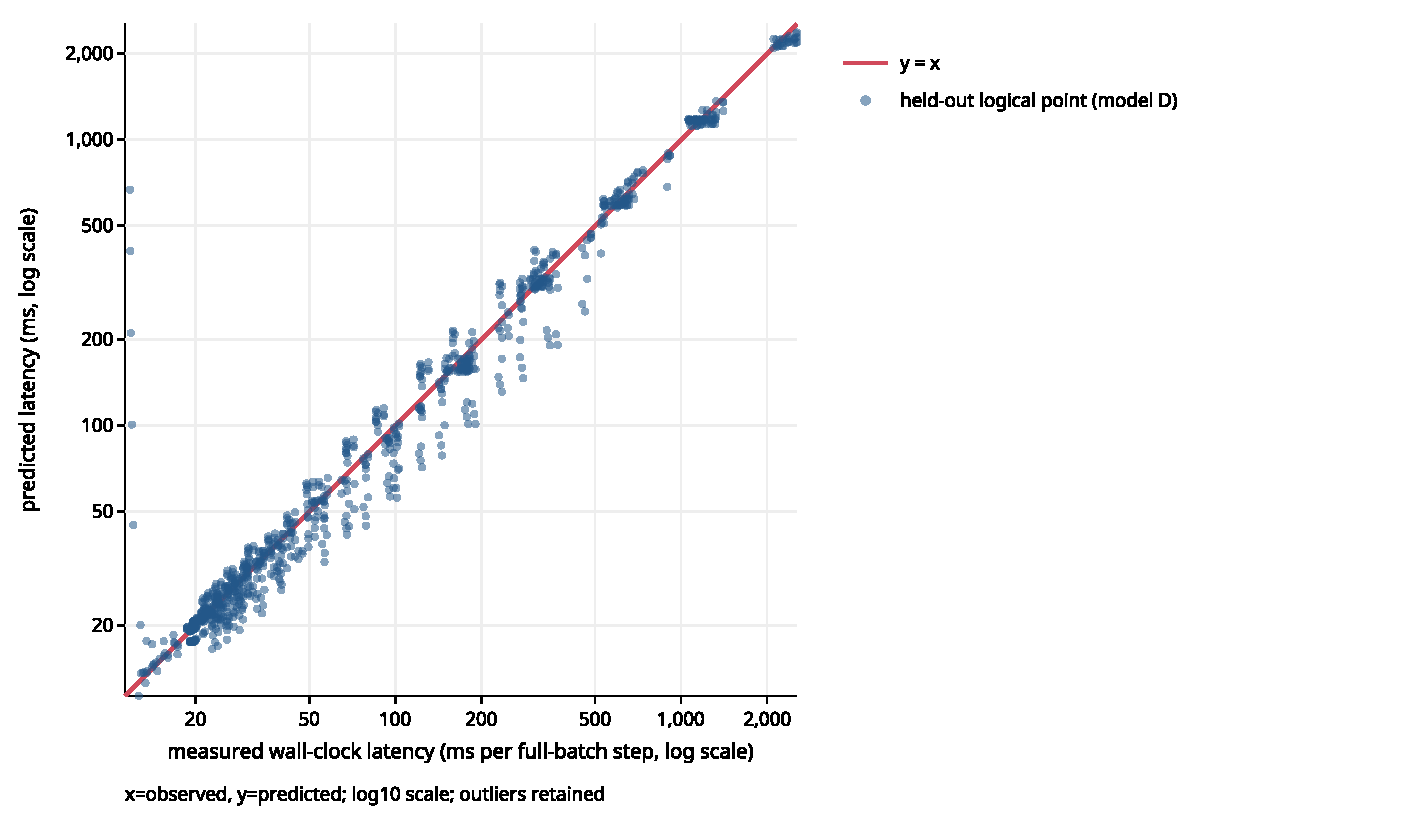
\includegraphics[width=0.8\textwidth]{figures/fig3_heldout_predicted_vs_measured.pdf}
\caption{Held-out predicted versus measured latency for model D over the three geometry holdout protocols (968 held-out predictions; both axes in ms on a log scale; red line $y = x$).
The vertical column at the far left is the BF16 batch-edge extrapolation failure, which is retained.}
\label{fig:heldout}
\end{figure*}

Of 50 configuration--batch curves, 23 have a knee identified within the measured range; 14 are weakly identified, 12 prefer a linear or constant description, and 1 has insufficient feasible span.
Intervals come from 1,000 bootstrap draws over the five process sessions.
Within the measured domain D interpolates reasonably for these ten configurations: held-out context bands give median errors of 1.8--9.7\%, and BF16 interior batch sizes give 2.5\% median and 6.0\% P95 error.
Outside it---batch sizes at the grid edge, quantizers beyond the three measured per family, other models, GPUs, or serving systems---the model is unvalidated, and its 67\% ranking accuracy makes it unsuitable for automatic method selection.
The evidence favors method-conditioned $B$/$L$/$r$ structure over a scalar byte law and leaves open whether $B$, $L$, and $r$ are sufficient.

\section{KVQuant quality and exclusion}
\label{app:kvquant}

\begin{table}[t]
\caption{KVQuant Fast perplexity versus BF16 (same protocol as Table~\mainref{tab:ppl}).
Intervals are paired 95\% CIs on $\Delta$NLL.}
\label{tab:kvq-ppl}
\vskip 0.1in
\centering
\scriptsize
\setlength{\tabcolsep}{2.5pt}
\begin{tabular}{@{}l>{\raggedleft\arraybackslash}p{1.95cm}>{\raggedleft\arraybackslash}p{1.05cm}lL{0.8cm}@{}}
\toprule
Configuration & Fast $\Delta$NLL \mbox{[95\% CI]} & Fast rel.\ PPL & Fast status & Full status \\
\midrule
KVQuant-4 & 3.397\newline \mbox{[3.297, 3.500]} & +2,888\% & FAIL & not run \\
KVQuant-3 & 3.387\newline \mbox{[3.288, 3.489]} & +2,859\% & FAIL & not run \\
KVQuant-2 & 3.411\newline \mbox{[3.319, 3.506]} & +2,930\% & FAIL & not run \\
\bottomrule
\end{tabular}
\end{table}

Perplexity rises about thirtyfold for all three KVQuant configurations, consistently across both datasets and all four lengths in the paired per-anchor data (Table~\ref{tab:kvq-ppl}).
These configurations produce finite outputs, pass cache-dependence controls, and match their method's reference fixtures, so the degradation is not a crash or numerical overflow.
Because it does not shrink from 2 to 4 bits, it is inconsistent with quantization error and points to a defect in the integrated port---the GQA/RoPE compatibility patch, the project-defined outlier capacity, the graph-safe and deterministic kernels, or the 16-window calibration of Section~\mainref{sec:impl}---whose cause we did not establish; it should not be attributed to KVQuant implementations in general.
After the results were known we therefore treat the result as invalid and exclude KVQuant from the quality conclusions.
The preregistered FAIL status in Table~\mainref{tab:joint} is unchanged, and the exclusion is recorded with the machine-readable reason \hash{quality\_result\_invalid\_suspected\_port\_defect} (root \anon{\texttt{47296f7c\ldots}}).
